\documentclass{beamer}

\usepackage{tikz}

\begin{document}

\begin{frame}{Serlo-Standorte}
    \centering
    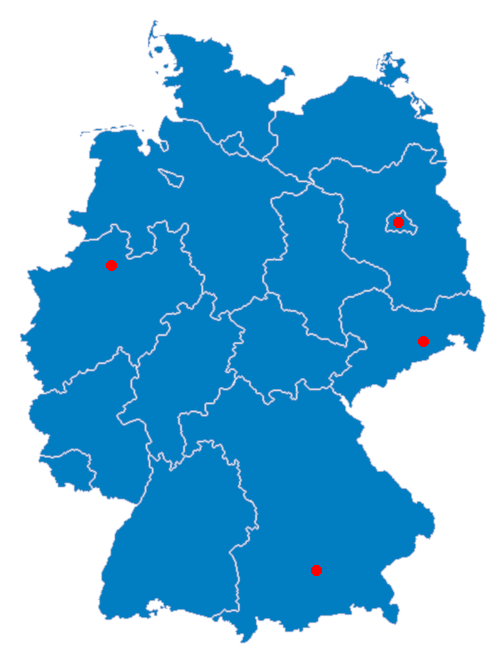
\includegraphics[height=0.8\textheight]{map.png}
    \begin{tikzpicture}[overlay]
        \node[anchor=east] (Berlin) at (2.4,4.96) {Berlin};
        \node[anchor=east] (Dresden) at (2.4,3.57) {Dresden};
        \node[anchor=east] (Munchen) at (2.4,0.88) {München};
        \node[align=left] (Munster) at (-8,4.46) {Münster};
        \draw[color=red] (Berlin.west) to (-1.26,4.96);
        \draw[color=red] (Dresden.west) to (-0.96,3.57);
        \draw[color=red] (Munchen.west) to (-2.25,0.88);
        \draw[color=red] (Munster.east) to (-4.7,4.46);
    \end{tikzpicture}
\end{frame}

\end{document}
